\documentclass{article}
\usepackage[sort, comma]{natbib}
\bibliographystyle{chicago2}
\usepackage[utf8]{inputenc}
\RequirePackage[left=1in, right=1in, top=1in, bottom=1in, headheight=12pt, letterpaper]{geometry}
\usepackage[utf8]{inputenc}
\usepackage[hyphens]{url}
\usepackage{xspace}
\usepackage{eucal}
\usepackage{geometry}
\usepackage{graphicx}
\usepackage{amsmath}
\usepackage{float}
\usepackage{verbatim}
\usepackage{fancyvrb}
\usepackage{longtable}
\usepackage{tabularx}
\usepackage{colortbl}
\usepackage{booktabs}
\usepackage{arydshln}
\usepackage{pdflscape}
\usepackage{afterpage}
\usepackage[colorlinks=true, citecolor = blue, linkcolor = black]{hyperref}
\usepackage{environ}
\usepackage{marginnote}
\usepackage{lineno}
\usepackage{setspace}
\usepackage{arydshln}
\usepackage{lscape}
\usepackage{palatino}
\usepackage{subfiles}
\usepackage{lscape} 
\usepackage{caption}
\usepackage{subcaption}
\usepackage{multirow}
\usepackage[english]{babel} 
\usepackage{xcolor}
\definecolor{vlg}{rgb}{0.88, 0.88, 0.88}
\newcolumntype{R}[1]{>{\raggedright\let\newline\\\arraybackslash\hspace{0pt}}m{#1}}
\newcommand{\alphastar}{\ensuremath{\alpha^{*}}}
\newcommand{\betaf}{\ensuremath{\beta_{f}}}
\newcommand{\betar}{\ensuremath{\beta_{r}}}
\newcommand{\mk}[1]{{\bf \color{red} MK: #1}}
\newcommand{\bb}[1]{{\bf \color{blue} BMB: #1}}
\newcommand{\jw}[1]{{\bf \color{green} JW: #1}}
\newcommand{\rzero}{{\cal R}_0\xspace}
\newcommand{\Reff}{{\cal R}_E\xspace}
\newcommand{\figref}[1]{Figure~\ref{fig:#1}}
\pagenumbering{gobble}

\title{Supplemental results for: The evolution of parasites constrained by a virulence-transmission tradeoff and compensatory virulence factor ``tuning''}
\author{Morgan P Kain\textsuperscript{1}* and Benjamin M Bolker\textsuperscript{1,2}}
\date{}

\begin{document}

\maketitle

\noindent *Corresponding author: kainm@mcaster.ca \\
\textsuperscript{1}Department of Biology, McMaster University, 1280 Main Street West, L8S 4K1 Hamilton, ON, Canada \\
\textsuperscript{2}Department of Mathematics and Statistics, McMaster University, 1280 Main Street West, L8S 4K1 Hamilton, ON, Canada \\

\clearpage

\setcounter{table}{0}
\renewcommand{\thetable}{S\arabic{table}}
\setcounter{section}{3}

\setcounter{figure}{0}
\renewcommand{\thefigure}{S\arabic{figure}}
\setcounter{section}{3}

\section*{Figures}

\subsection*{Parasite evolution from high virulence low efficiency}

\begin{figure}[H]
\makebox[\textwidth][c]{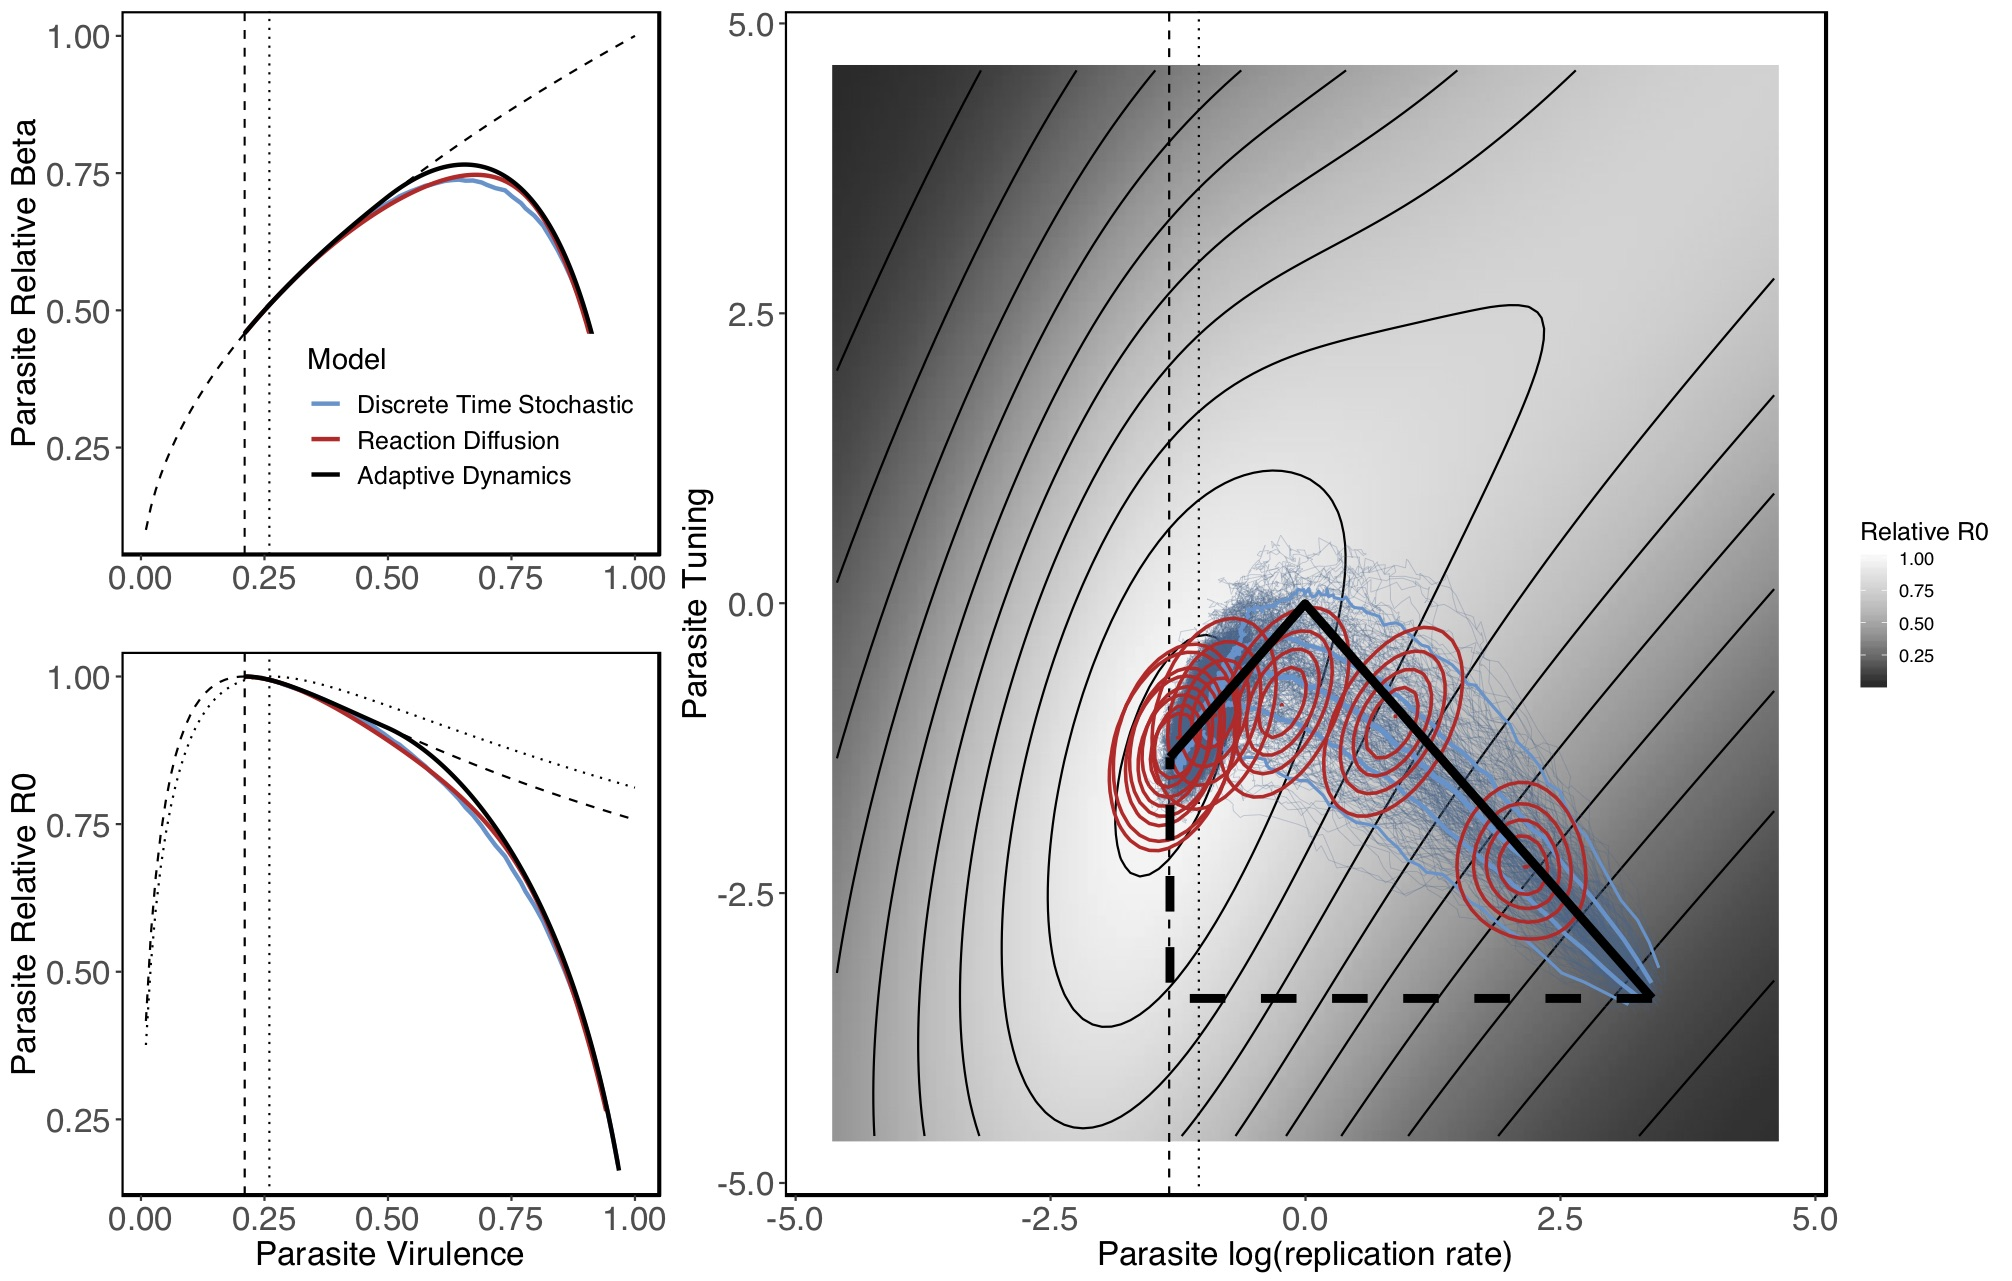
\includegraphics[width=1.0\textwidth]{Supp_Figures/landscape1_br.jpg}}
\caption{The large right panel shows the evolutionary trajectory of a parasite on its fitness landscape in the DTS model (thin blue lines show 250 stochastic simulations, while the solid blue lines show the median, 50\%, and 95\% quantities of these simulations), RD model (red ellipses show 95\% of the distribution of parasite strains), and AD model (bold black solid line shows simultaneous evolution in two traits; dashed lines show evolution in a single trait per time step), using the same parameter values as main text Figure~1, except here parasites evolve from high replication rate and low tuning. The surface pictured is calculated using the $\rzero$ equation for rates (Eq.1), and has been scaled so that the adaptive peak has a value of 1 (shown in light grey). Due to the slight difference in $\rzero$ for the RD and DTS models (Eq.2 vs Eq.3), the DTS surface is marginally different (see Figure S3 for a comparison of these surfaces). The thin dashed vertical line shows the location of the adaptive peak for this surface; the thin dotted vertical line shows the location of the peak for the DTS model. 
\break
The top left and bottom left panels show a parasite evolving in log(replication rate) and tuning, according to the right panel, translated into virulence and transmission following a power-law tradeoff (top panel) and virulence and $\rzero$ (bottom panel). The dashed curve in the bottom left panel shows parasite $\rzero$ for the RD and AD models; the dotted curves shows parasite $\rzero$ for the DTS model. Maximum $\rzero$ is designated by the vertical dashed and dotted lines respectively. All models have the same power-law tradeoff curve (top right panel).} 
\label{fig:landscape1_br}
\end{figure} 
\clearpage

\subsection*{Parasite evolution from low virulence and high efficiency}

\begin{figure}[H]
\makebox[\textwidth][c]{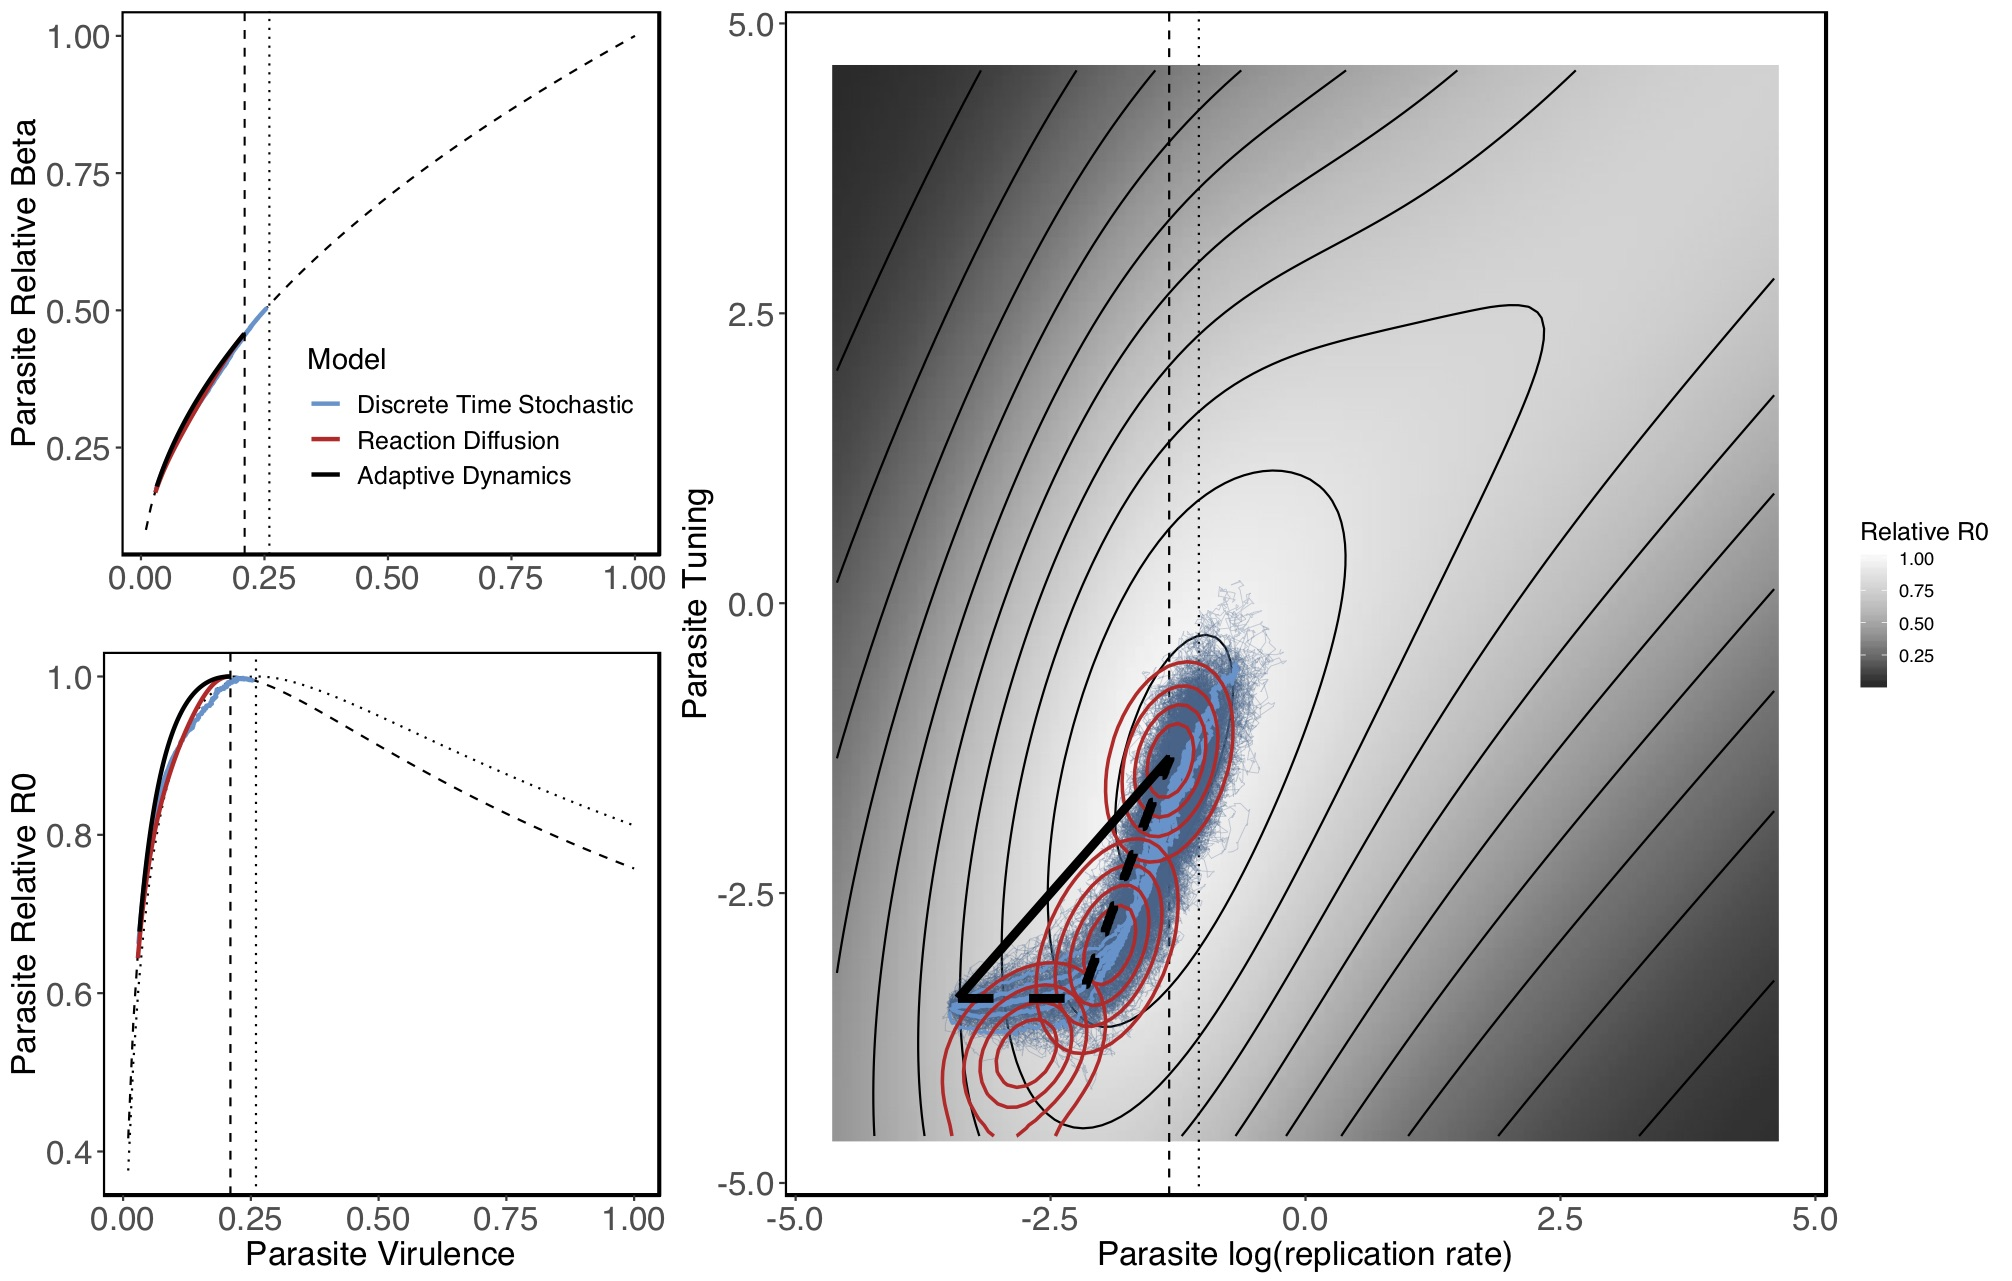
\includegraphics[width=1.0\textwidth]{Supp_Figures/landscape1_bl.jpg}}
\caption{For a complete figure caption see \figref{landscape1_br}. Panels show the evolutionary trajectory of a parasite in the DTS (blue lines), RD (red ellipses), and AD (black solid and dashed lines) models, using the same parameter values as main text Figure~1, except here parasites evolve from low replication rate and low tuning.} 
\label{fig:landscape1_bl}
\end{figure} 


\subsection*{Comparison of fitness landscapes}

\begin{figure}[H]
\makebox[\textwidth][c]{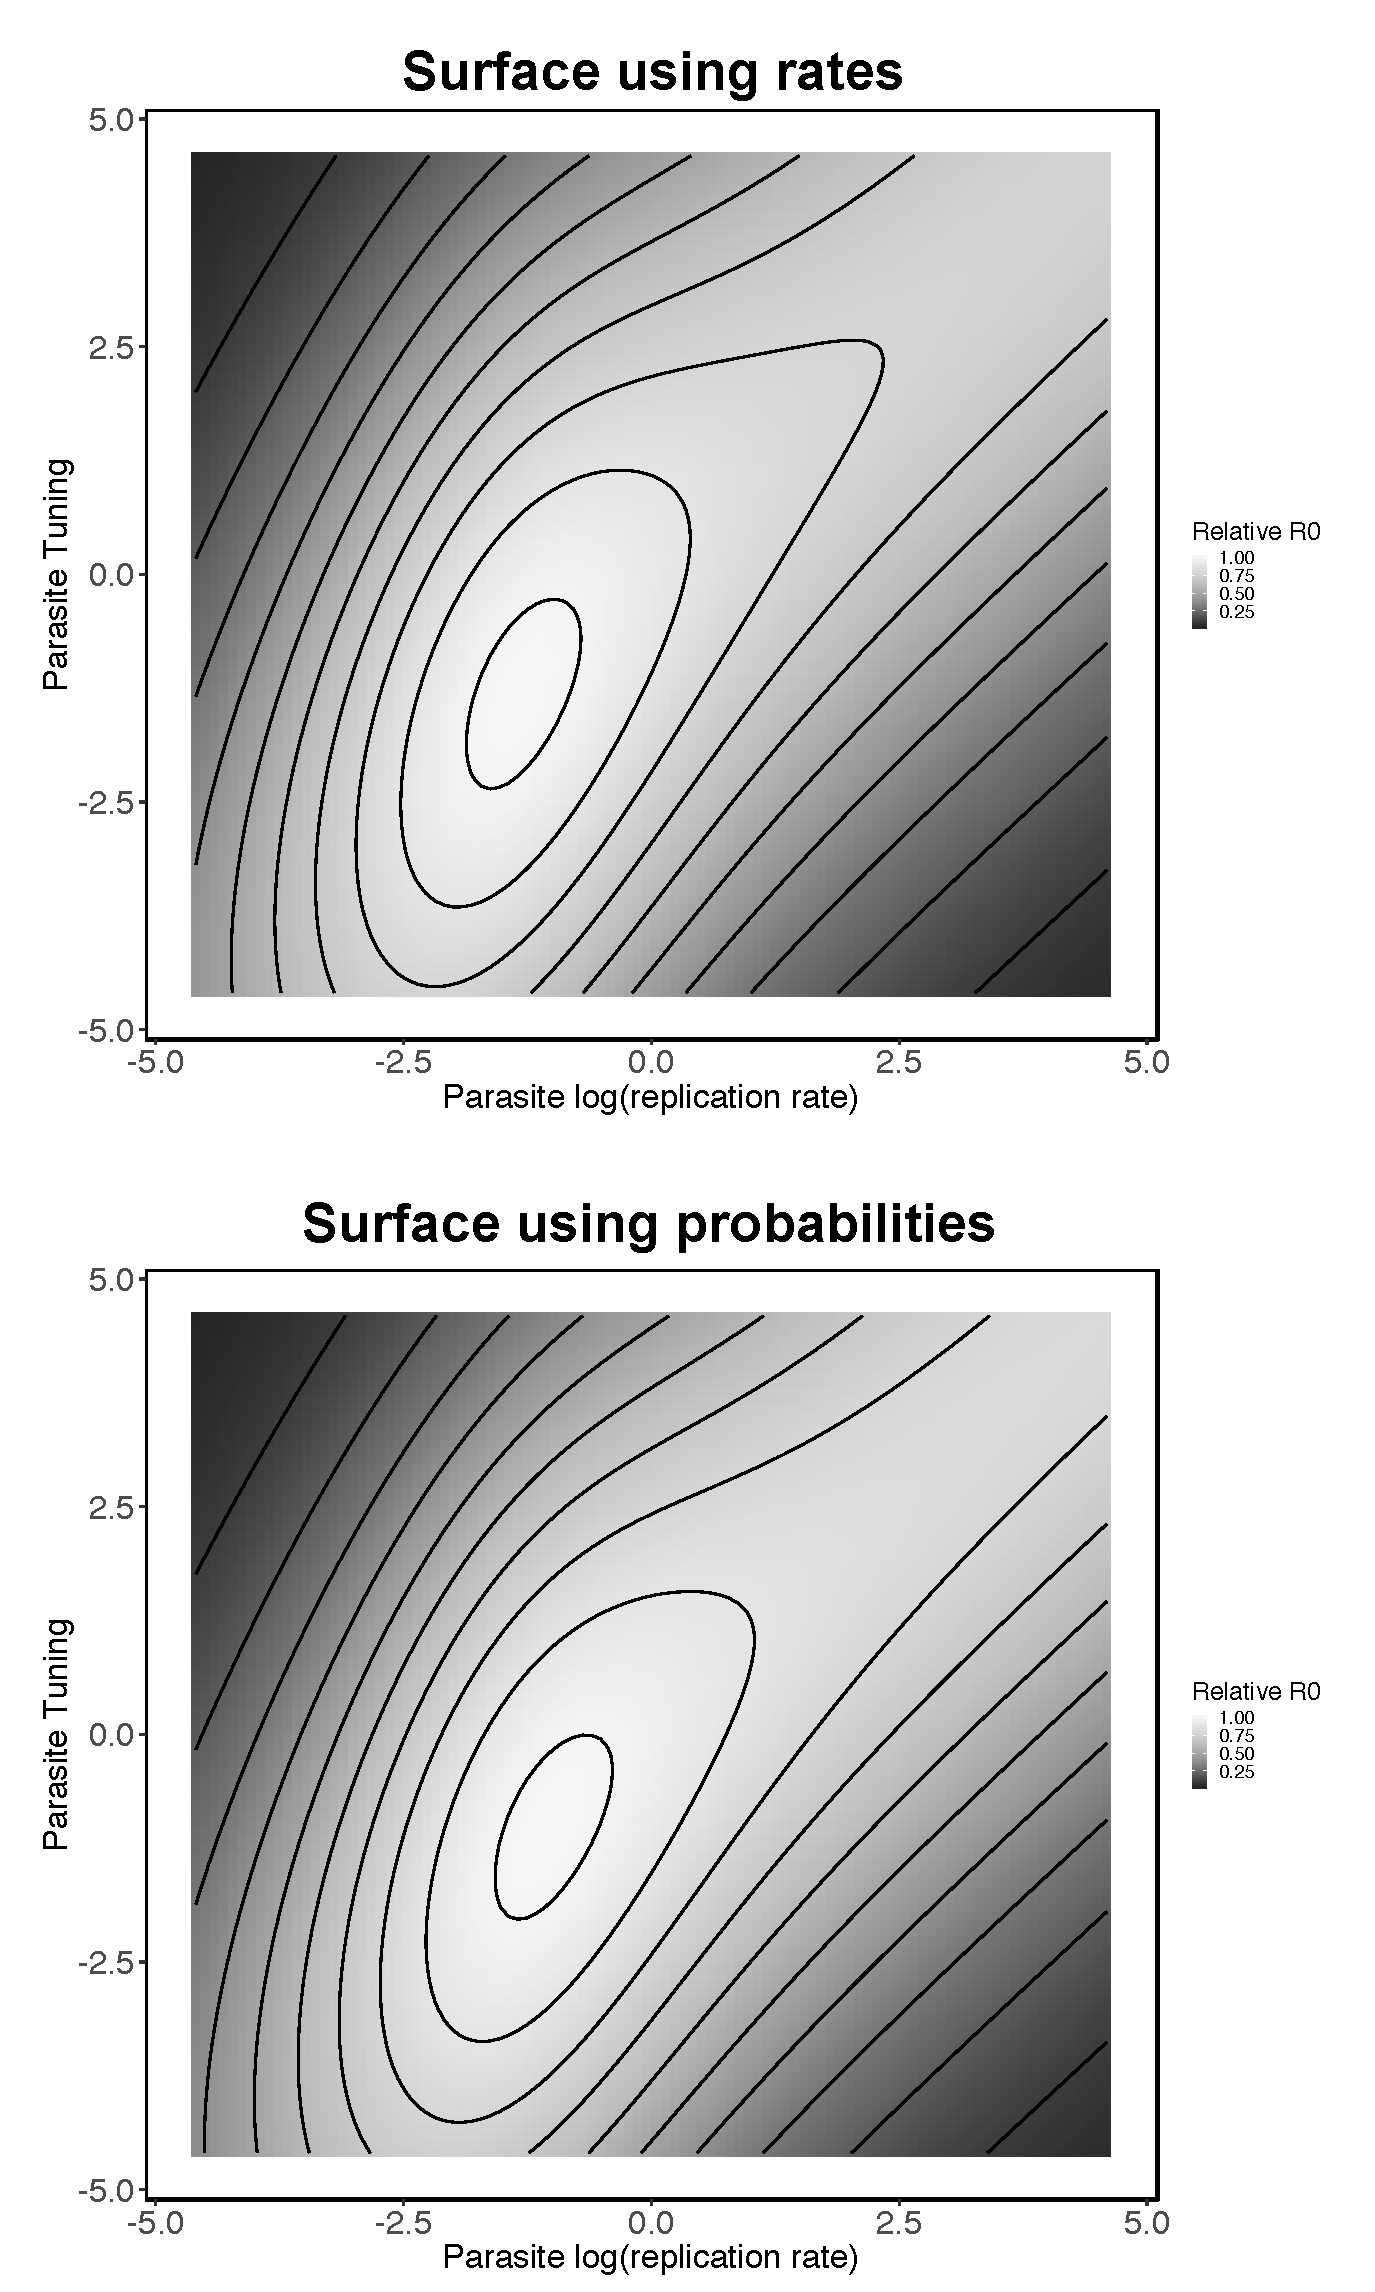
\includegraphics[width=0.8\textwidth]{Supp_Figures/surface_comparison.pdf}}
\caption{Top and bottom panels show a fitness landscape with rates (Main text Eq.2) and probabilities (Main text Eq.3) respectively using recovery ($\gamma$) of 0.2 and a background death ($\mu$) of 0.01. Parasite optimal virulence in the top panel is 0.21 and 0.26 in the bottom panel.} 
\label{fig:surface_comparison}
\end{figure} 
\clearpage

\subsection*{DTS dynamics when a parasite evolves from high virulence and low efficiency}

\begin{figure}[H]
\makebox[\textwidth][c]{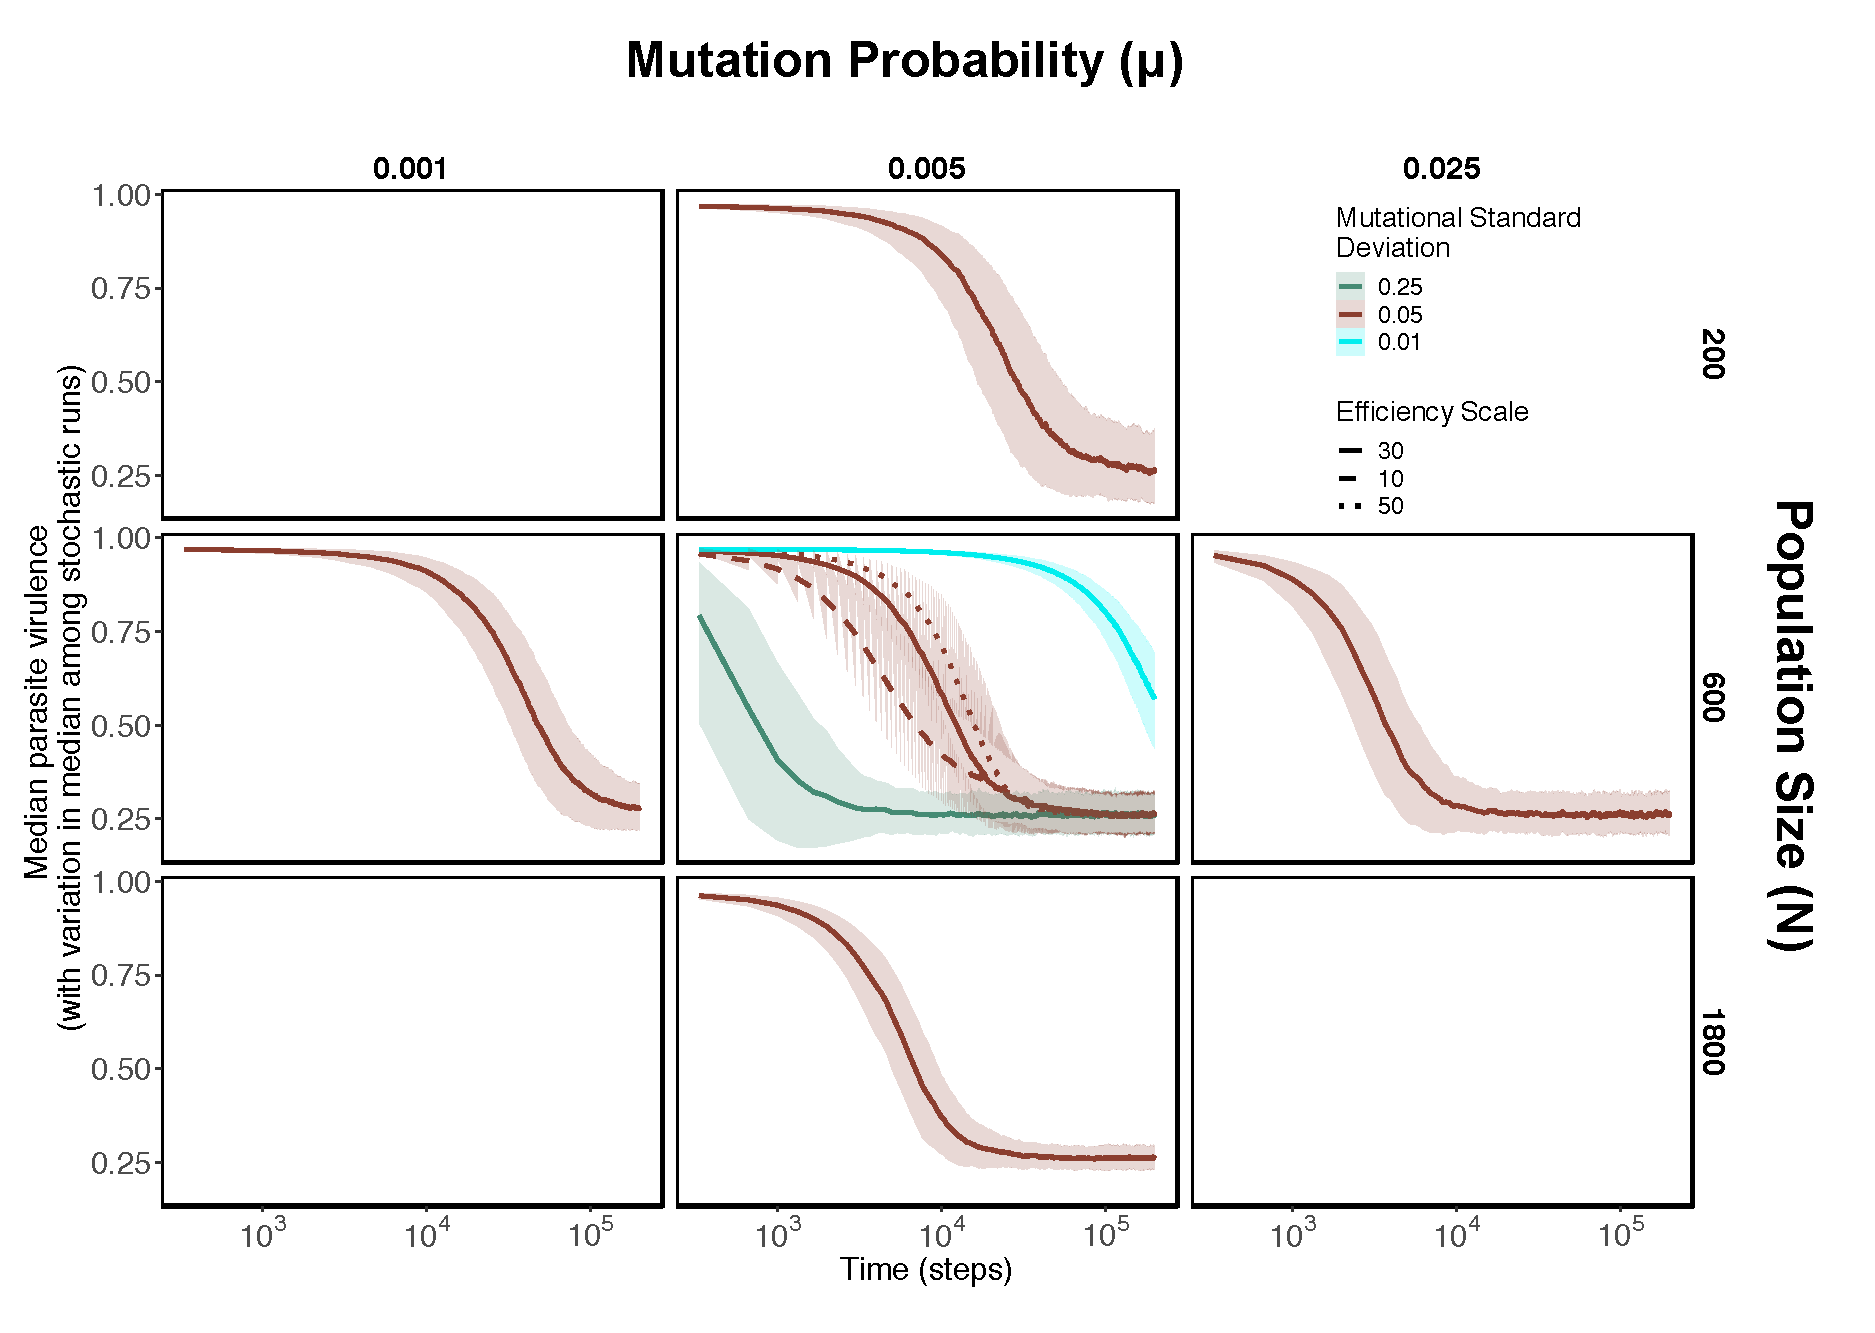
\includegraphics[width=1.0\textwidth]{Supp_Figures/DTS_results1br.pdf}}
\caption{Parasite virulence for all parameter combinations presented in Table~2 for a parasite evolving from high virulence and low efficiency. Bold lines represent medians across 250 stochastic simulations; shaded envelopes show the 95\% quantiles. The correspondence between each ``Model Outcome'' presented in Table~2, from left to right, are as follows: 1) Median number of circulating strains: not pictured; 2) Time to optimum virulence: Time at which median virulence first reaches 0.26; 3) Maximum transient virulence: not relevant for these starting values; 4) Time with greater than optimum virulence: same as time to optimum virulence for these starting values; 5) Departure from optimum virulence: width of the shaded envelope once a virulence of 0.26 is reached.)} 
\label{fig:DTS1br}
\end{figure} 
\clearpage

\subsection*{Parasite evolution with high mutational standard deviation}

\begin{figure}[H]
\makebox[\textwidth][c]{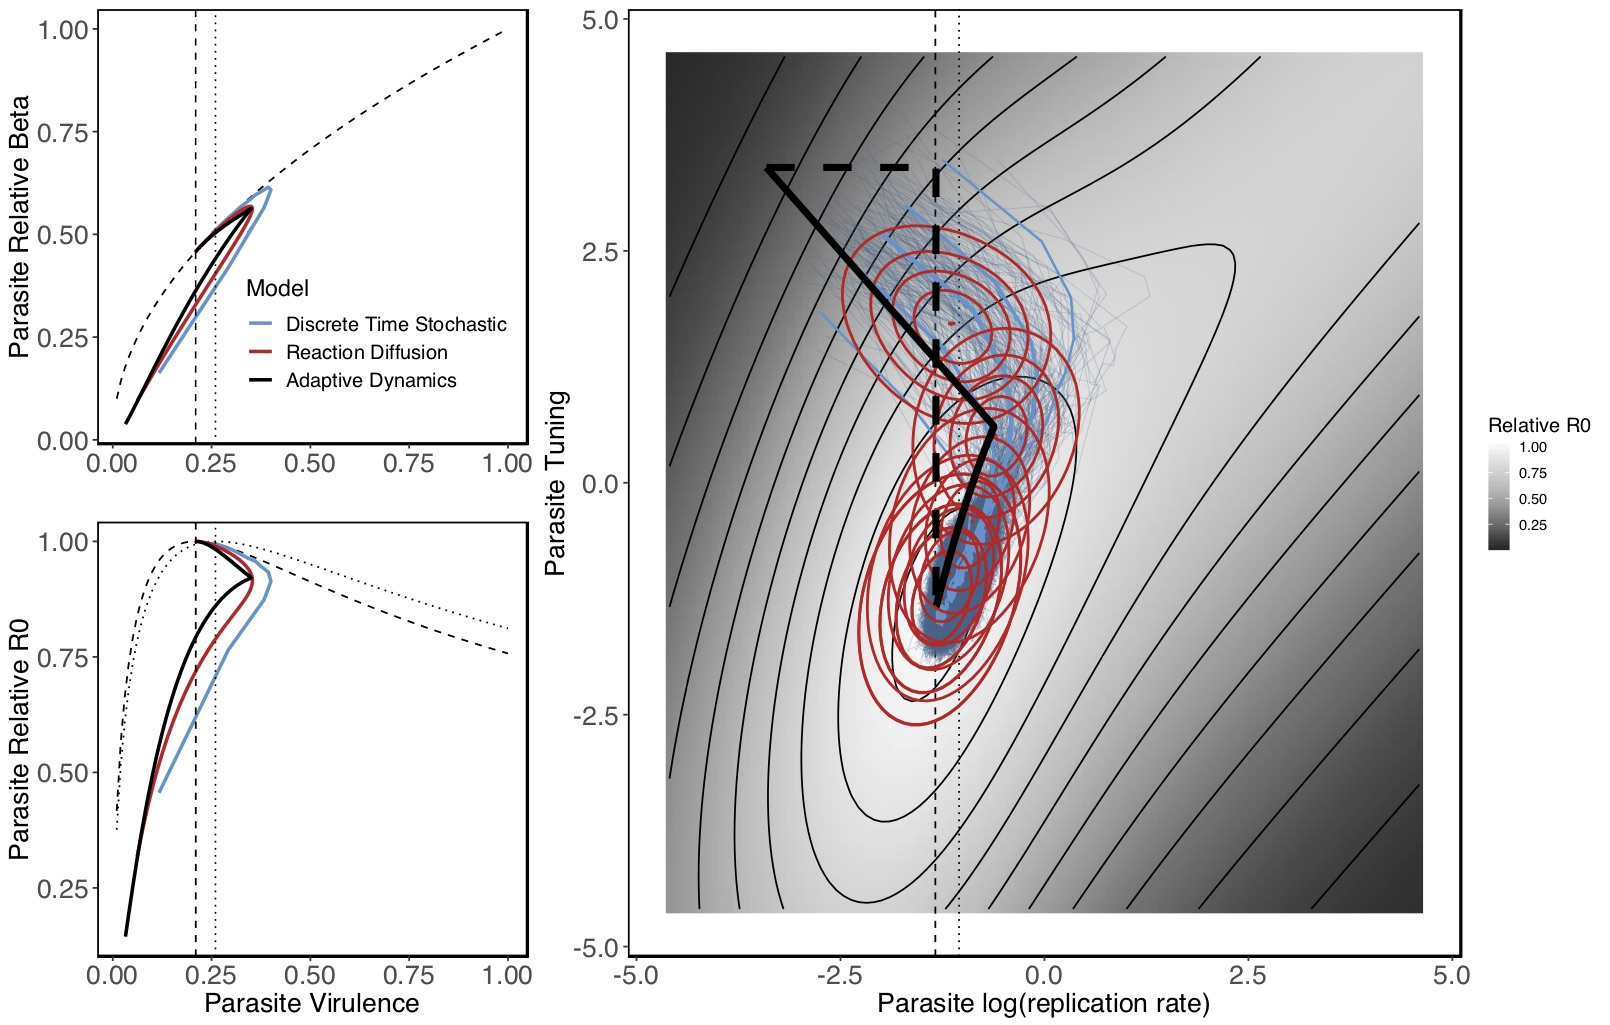
\includegraphics[width=1.0\textwidth]{Supp_Figures/landscape1_high_var.jpg}}
\caption{For a complete figure caption see \figref{landscape1_br}. Panels show the evolutionary trajectory of a parasite in the DTS (blue lines), RD (red ellipses), and AD (black solid and dashed lines) models, using the same parameter values as main text Figure~1, except with: DTS: $\sigma = 0.25$; RD: $\sigma = 0.39$. A numeric summary of the DTS model for these parameter values is available in main text Table~2 row~5.} 
\label{fig:landscape1_high_var}
\end{figure} 
\clearpage

\subsection*{Parasite evolution with a small population size}

\begin{figure}[H]
\makebox[\textwidth][c]{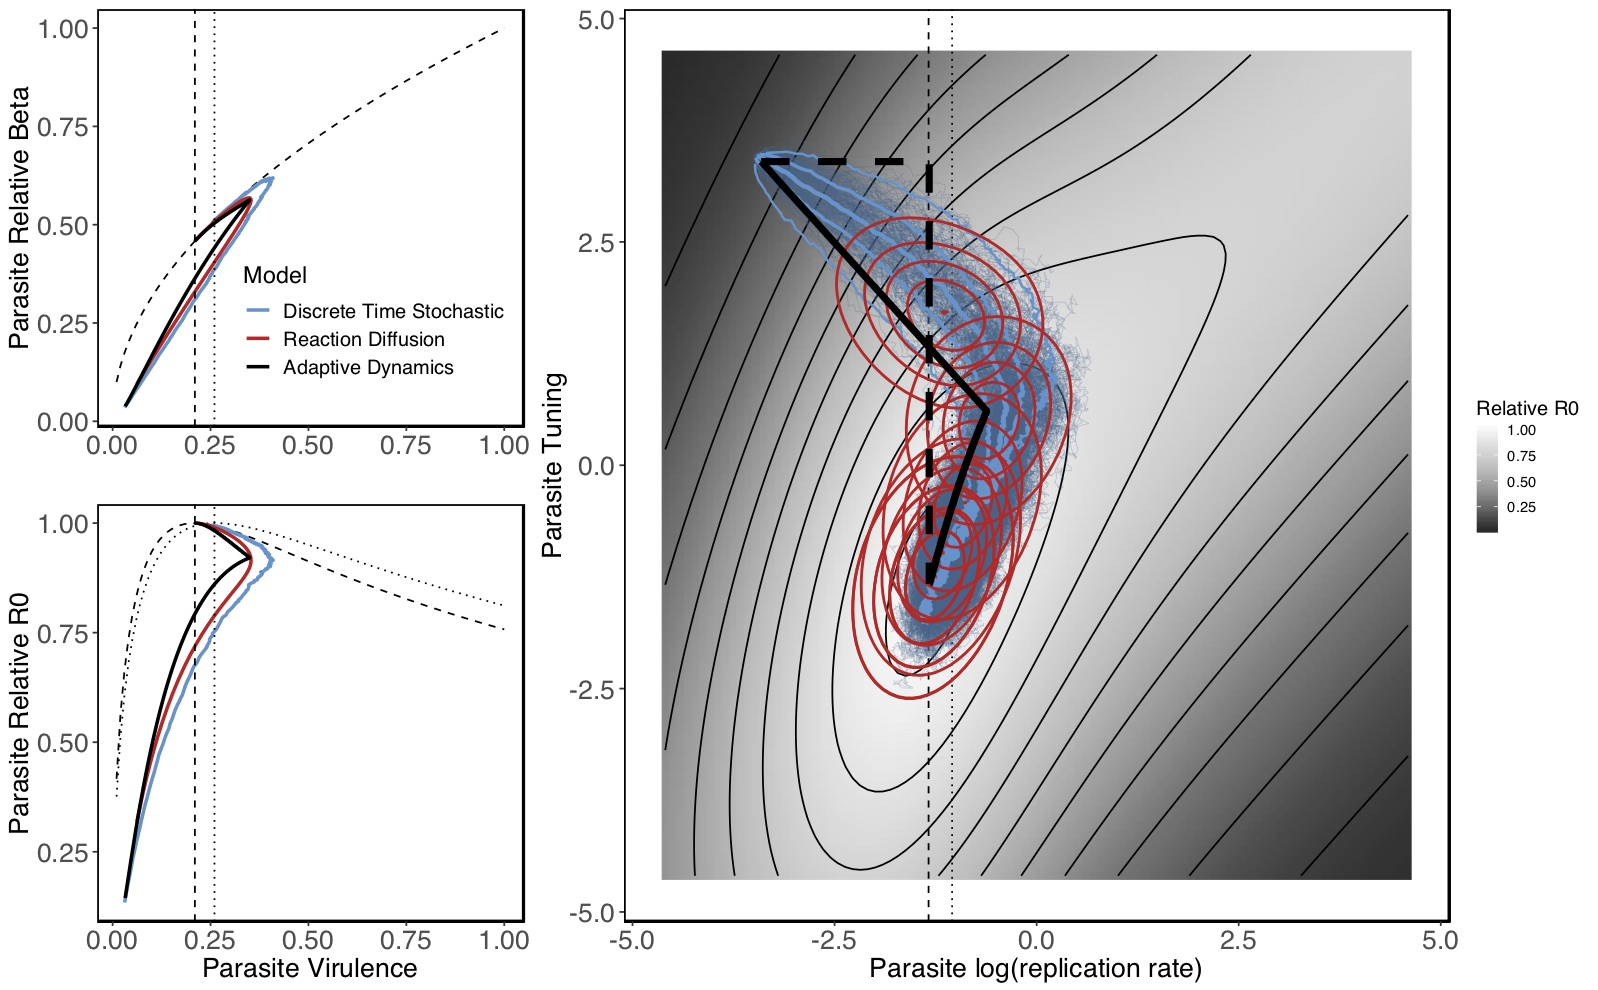
\includegraphics[width=1.0\textwidth]{Supp_Figures/landscape1_small_pop.jpg}}
\caption{For a complete figure caption see \figref{landscape1_br}. Panels show the evolutionary trajectory of a parasite in the DTS (blue lines), RD (red ellipses), and AD (black solid and dashed lines) models, using the same parameter values as main text Figure~1, except with N = 200. A numeric summary of the DTS model for these parameter values is available in Table~2 row~7.} 
\label{fig:landscape1_small_pop}
\end{figure} 
\clearpage






\end{document}
